\chapter{Υλοποιήσεις}
\label{chapter:implementations}

Η παρούσα διπλωματική εργασία καταπιάνεται με το
πρόβλημα της ανάπτυξης νευρωνικών δικτύων στην πλατφόρμα Jetson TK1
και στοχεύει στην ανάπτυξη ενός νευρωνικού δικτύου για ταυτόχρονη
αναγνώριση και εντοπισμό αντικειμένων (object detection) σε εικόνες.

Ένα CNN αποτελείται από πολλά επίπεδα συνέλιξης, τα οποία με την σειρά τους
αποτελούνται από εκατομμύρια νευρώνες το κάθε ένα. Αυτό σημαίνει και εκατομμύρια
παραμέτρους όπου η καθεμία είναι ένας αριθμός κινητής υποδιαστολής 32 bit.
Το ενσωματωμένο σύστημα Jetson TK1 έχει περιορισμένη χωρητικότητα μνήμης (2GB),
γεγονός που λήφθηκε υπόψη κατά την επιλογή των μοντέλων CNN που υλοποιήθηκαν.

Οι υλοποιήσεις χωρίζονται σε 2 μέρη:
\begin{itemize}
  \item{Ανάπτυξη διαφόρων μοντέλων CNN για αναγνώριση αντικειμένων σε εικόνες}
  \item{Ρυθμίσεις και βελτιστοποιήσεις στο Jetson TK1}
\end{itemize}

Στο πρώτο μέρος παρουσιάζονται και αναλύονται τα μοντέλα CNN που αναπτύχθηκαν, ενώ στο
δεύτερο δίνεται μία πλήρης περιγραφή των διαδικασιών ρύθμισης και βελτιστοποίησης που έγιναν
στο ενσωματωμένο σύστημα Jetson TK1 καθώς και τα εργαλεία που χρειάστηκε να εγκατασταθούν.

\section{Μοντέλα CNN}
\label{sec:cnn_impl}

Όπως αναφέραμε \autoref{sec:dnn_sw} το βασικό εργαλείο λογισμικού που
χρησιμοποιήσαμε για την ανάπτυξη των μοντέλων CNN είναι το \emph{Keras}.

Η βιβλιοθήκη Keras προσφέρει τις υλοποιήσεις όλων των επιπέδων που
απαιτούνται για για την ανάπτυξη ενός CNN
\footnote{Πλήρες περιγραφή της λίστας των διαθέσιμων επιπέδων: \href{https://keras.io/layers/core/}{https://keras.io/layers/core/}}.
Πιο συγκεκριμένα, τα επίπεδα που χρησιμοποιήθηκαν, καθώς και οι βασικές
παράμετροι τους περιγράφονται πιο κάτω:
\begin{itemize}
  \item{\textbf{InputLayer}: Επίπεδο Εισόδου του νευρωνικού δικτύου}
    \begin{itemize}
      \item{Διαστάσεις του όγκου εισόδου (tensor shape)}
    \end{itemize}
  \item{Convolution2D: Επίπεδο Συνέλιξης}
    \begin{itemize}
      \item{Μορφολογία της εισόδου}
      \item{Αριθμός των φίλτρων συνέλιξης}
      \item{Διαστάσεις των φίλτρων συνέλιξης}
      \item{Συνάρτηση ενεργοποίησης}
    \end{itemize}
  \item{MaxPooing2D: Επίπεδο Υποδειγματοληψίας}
    \begin{itemize}
      \item{Διαστάσεις πλαισίου}
      \item{Βήμα μετατόπισης}
    \end{itemize}
  \item{ZeroPadding2D: Προσθέτει πλαίσιο με μηδενικά στον όγκο εισόδου}
    \begin{itemize}
      \item{Διαστάσεις του πλαισίου}
    \end{itemize}
  \item{Activation: Επίπεδο ενεργοποίησης. Εφαρμόζει συνάρτηση ενεργοποίησης στον
    όγκο εξόδου του προηγούμενου επιπέδου}
  \item{Dropout: Επίπεδο πρόληψης υπέρ-προσαρμογής \cite{lecun2015deep}}
  \item{Dense: Πλήρες συνδεδεμένο επίπεδο}
    \begin{itemize}
      \item{Διαστάσεις του όγκου εισόδου (Προαιρετικό)}
      \item{Διαστάσεις του όγκου εξόδου}
      \item{Συνάρτηση ενεργοποίησης}
    \end{itemize}
  \item{Flatten: Μετασχηματίζει τον όγκου εισόδου σε επίπεδη αναπαράσταση
    (π.χ. για όγκο εισόδου $64 \times 32 \times 32$ η έξοδος θα είναι επίπεδη με $65536$ νευρώνες}
  \item{BatchNormalization: Εφαρμόζει μετασχηματισμό για να κρατήσει την μέση τιμή
      και την τυπική απόκλιση των ενεργοποιήσεων του προηγούμενου επιπέδου στις τιμές 0 και 1 αντίστοιχα}
\end{itemize}

Σημαντική παρατήρηση είναι το γεγονός ότι η επιστήμη της βαθιάς μηχανικής μάθησης
βρίσκεται σε πρώιμο στάδιο, με αποτέλεσμα να μην υπάρχουν συγκεντρωμένες
οι υλοποιήσεις των διαφόρων επιπέδων και γενικότερα των μοντέλων σύγχρονων ΑNN.

Περαιτέρω, η επιλογή των μοντέλων CNN για ανάπτυξη στηρίχθηκε στην ύπαρξη και
προ-εκπαιδευμένων βαρών για τα αντίστοιχα CNN στο διαδίκτυο για 2 λόγους:
\begin{itemize}
  \item{Η διαδικασία εκπαίδευσης είναι χρονοβόρα διαδικασία και προϋποθέτει
    τη χρησιμοποίηση μίας ή περισσοτέρων ισχυρών μονάδων GPU (NVIDIA Titam X GPU)}
  \item{Η εκπαίδευση νευρωνικών δικτύων ξεφεύγει από τα πλαίσια της παρούσας
    διπλωματικής εργασίας}
\end{itemize}


\subsection{AlexNet}

Το δίκτυο AlexNet ήταν η αρχή της εισαγωγής της βαθιάς
μηχανικής μάθησης στην επιστήμη της μηχανικής όρασης. Εμφανίστηκε και χρησιμοποιήθηκε
στον διαγωνισμό ImageNet ILSVRC challenge, το 2012, κερδίζοντας με διαφορά
10,9\%, στο σφάλμα αναγνώρισης αντικειμένων σε σύνολο 1000 κλάσεων.

\begin{figure}[!ht]
  \centering
  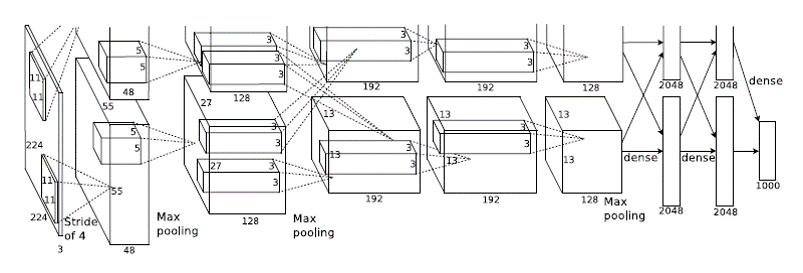
\includegraphics[width=1\textwidth]{./images/chapter5/alexnet_from_paper.png}
  \caption[Μοντέλο δικτύου AlexNet]{%
    Μοντέλο δικτύου AlexNet \\
    Πηγή: Άρθρο δημοσίευσης \emph{ImageNet Classification with Deep Convolutional Neural Networks} \cite{NIPS2012_4824}
  }
  \label{fig:alexnet_from_paper}
\end{figure}

Το συγκεκριμένο νευρωνικό δίκτυο συνέλιξης αποτελείται από σύνολο οκτώ επίπεδα,
ή καλύτερα ομάδες επιπέδων; πέντε επίπεδα συνέλιξης και 3 πλήρως συνδεδεμένα. \\

\begin{tabular}{ | l | l | l | l | }
  \hline
  \rowcolor{Gray}
  Επίπεδο  & Τύπος & Αριθμός καναλιών & Διαστάσεις φίλτρων \\
  \hline
  1 & Conv+Pool+Norm & 96 & $11 \times 11$ \\
  2 & Conv+Pool+Norm & 256 & $5 \times 5$ \\
  3 & Conv & 384 & $3 \times 3$ \\
  4 & Conv & 384 & $3 \times 3$ \\
  5 & Conv+Pool & 256 & $3 \times 3$ \\
  6 & Full & 4096 & Ν/A \\
  7 & Full & 4096 & N/A \\
  8 & Full & 1000 & N/A \\
  \hline
\end{tabular}
\\

Η συνάρτηση υποδειγματοληψίας που χρησιμοποιεί το μοντέλο είναι η συνάρτηση
MaxPooling2D με βήμα μετατόπισης ίσο με την μονάδα και στους 2 άξονες ($1 \times 1$).
Σε όλα τα επίπεδα εκτός του τελευταίου χρησιμοποιήθηκε η συνάρτηση ενεργοποίησης
ReLU. Επίσης χρησιμοποιεί και πολλά επίπεδα ZeroPadding με πλαίσιο
διαστάσεων $1 \times 1$. Το τελευταίο επίπεδο παίζει τον ρόλο του ταξινομητή και συγκεκριμένα
είναι ένας ταξινομητής Softmax.

Η υλοποίηση στηρίχτηκε στην αντίστοιχη που υπάρχει με το εργαλείο Caffe
\footnote{Υλοποίηση του δικτύου AlexNet στο Caffe: \url{https://github.com/BVLC/caffe/tree/master/models/bvlc_alexnet}}.
Πρακτικά μεταφράστηκε ο πηγαίος κώδικας της υλοποίησης από το Caffe στο Keras.
Ο αντίστοιχος γράφος της υλοποίησης του μοντέλου
φαίνεται φαίνεται στο \autoref{fig:alexnet_2}.

\begin{figure}[!ht]
  \centering
  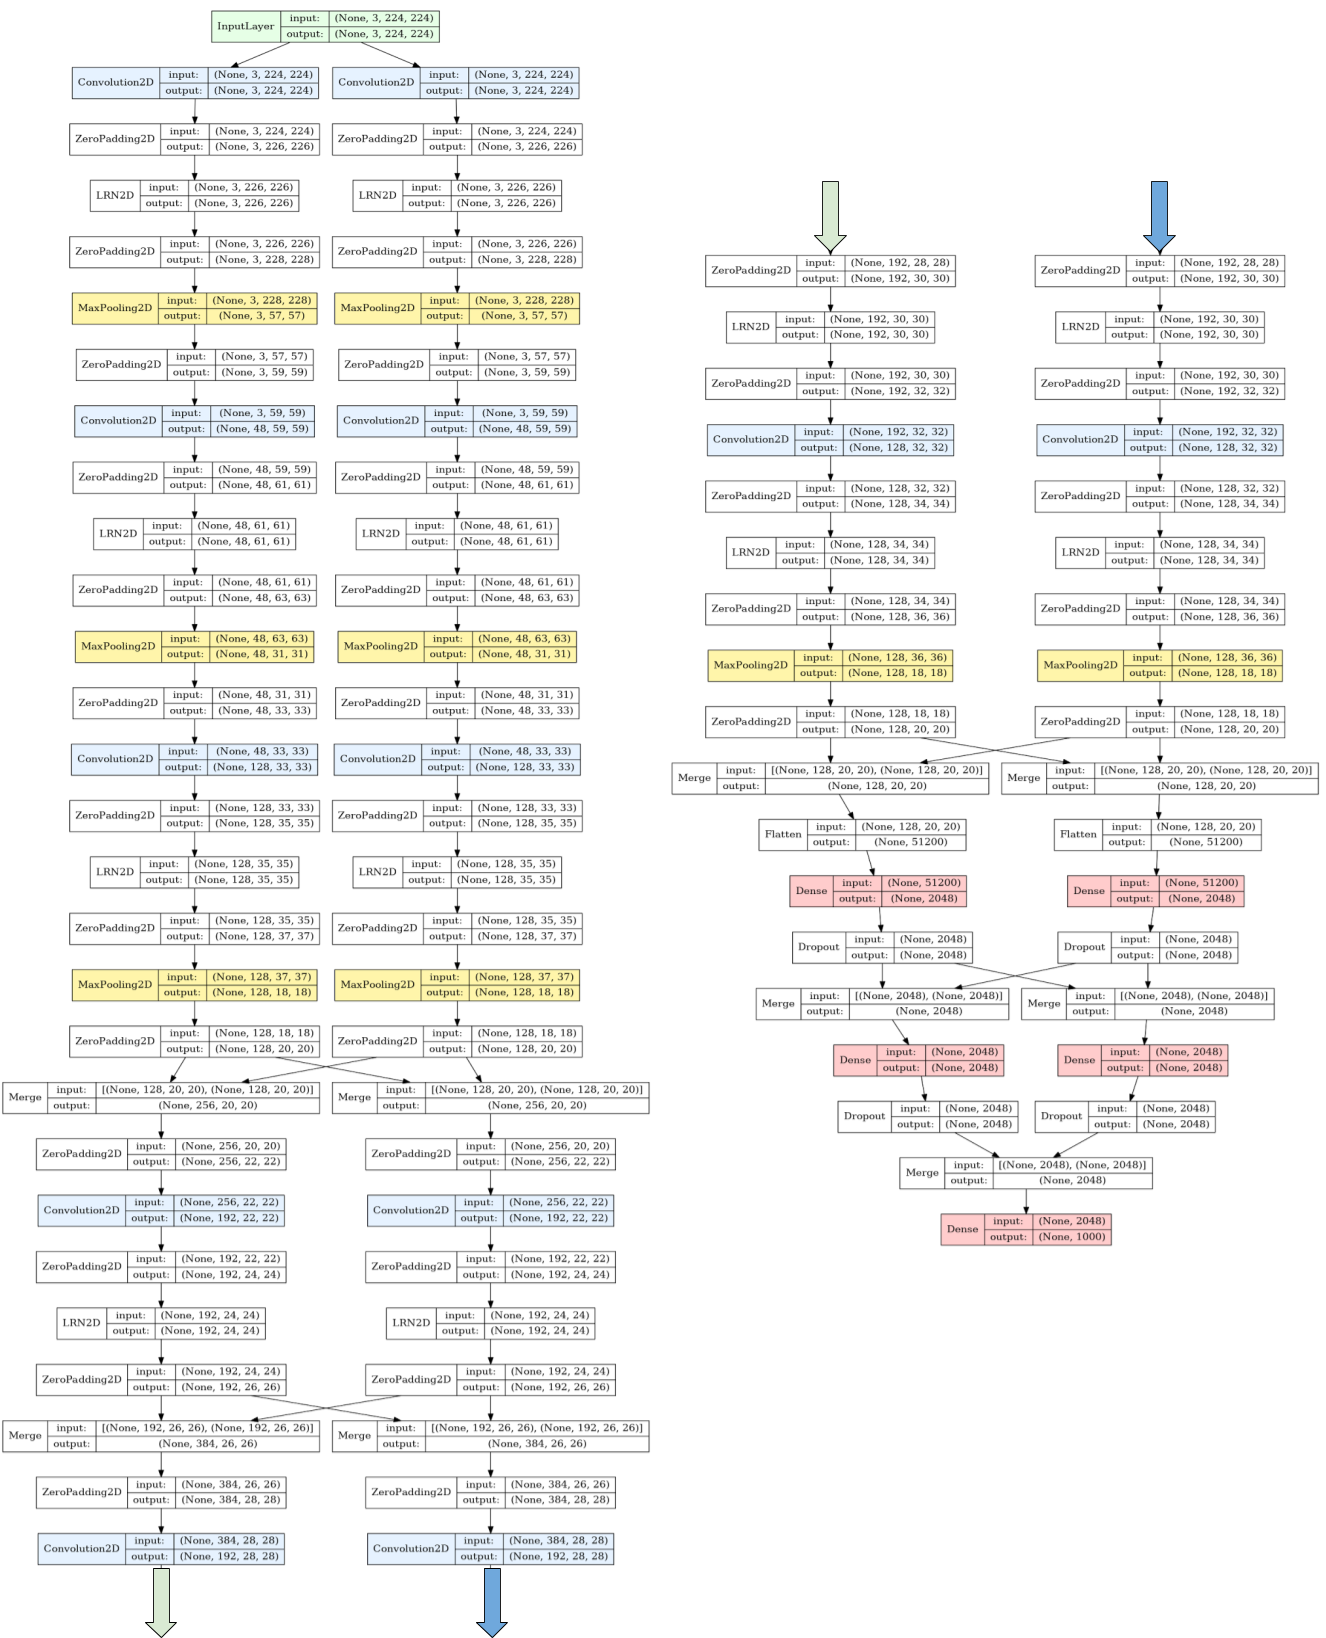
\includegraphics[width=1\textwidth]{./images/chapter5/alexnet_3.png}
  \caption[Πλήρες μορφή του δικτύου AlexNet της υλοποίησης]{Πλήρες μορφή του δικτύου AlexNet της υλοποίησης}
  \label{fig:alexnet_2}
\end{figure}

Το AlexNet είναι ένα μοντέλο μόνο για αναγνώριση και όχι για εντοπισμό
των αντικειμένων, δηλαδή η μόνη πληροφορία που μας δίνει είναι η κλάση των
αντικειμένων.

%% --------------------------------------------------------------------------
\subsection{VGG16}

Το δίκτυο VGG16 ήταν ο νικητής του διαγωνισμού ImageNet ILSVRC-2014 με σφάλμα
κατηγοριοποίησης 7.5\% σε σύνολο 1000 κλάσεων αντικειμένων \cite{Simonyan14c}.

\begin{figure}[!ht]
  \centering
  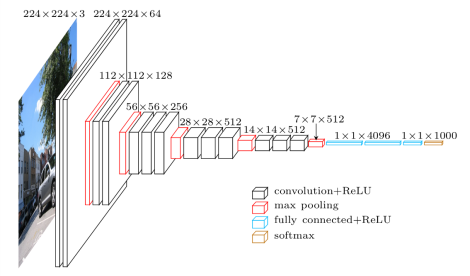
\includegraphics[width=0.8\textwidth]{./images/chapter5/vgg16_from_paper.png}
  \caption[Mορφή του δικτύου VGG16]{Μορφή του δικτύου VGG16}
  \label{fig:vgg16_from_paper}
\end{figure}

Αποτελείτε από 16 επίπεδα; 13 επίπεδα συνέλιξης και 3 πλήρως συνδεδεμένα (\autoref{fig:vgg16_from_paper}), των
οποίων τα χαρακτηριστικά δίνονται πιο κάτω:
\\

\begin{tabular}{ | l | l | l | l | }
  \hline
  \rowcolor{Gray}
  Επίπεδο  & Τύπος & Αριθμός καναλιών & Διαστάσεις φίλτρων \\
  \hline
  1 & Conv & 64 & $3 \times 3$ \\
  2 & Conv+Pool & 64 & $3 \times 3$ \\
  3 & Conv & 128 & $3 \times 3$ \\
  4 & Conv+Pool & 128 & $3 \times 3$ \\
  5 & Conv & 256 & $3 \times 3$ \\
  6 & Conv & 256 & $3 \times 3$ \\
  7 & Conv+Pool & 256 & $3 \times 3$ \\
  8 & Conv & 512 & $3 \times 3$ \\
  9 & Conv & 512 & $3 \times 3$ \\
  10 & Conv+Pool & 512 & $3 \times 3$ \\
  11 & Conv & 512 & $3 \times 3$ \\
  12 & Conv & 512 & $3 \times 3$ \\
  13 & Conv+Pool & 512 & $3 \times 3$ \\
  14 & FullyConnected & 4096 & Ν/A \\
  15 & FullyConnected & 4096 & N/A \\
  16 & FullyConnected & 1000 & N/A \\
  \hline
\end{tabular}
\\

Παρόμοια με το δίκτυο AlexNet, σε όλα τα επίπεδα εκτός του τελευταίου χρησιμοποιήθηκε η συνάρτηση ενεργοποίησης
ReLU, ενώ το τελευταίο επίπεδο παίζει τον ρόλο του ταξινομητή και συγκεκριμένα
είναι ένας ταξινομητής Softmax. Το βήμα μετατόπισης των συναρτήσεων υποδειγματοληψίας
είναι διαστάσεων $1 \times 1$.

Το μοντέλο του δικτύου VGG16 υπάρχει υλοποιημένο στην λίστα με τα παραδείγματα
του εργαλείου Keras \footnote{\url{https://github.com/fchollet/keras/tree/master/keras/applications}}.
Ο αντίστοιχος γράφος της υλοποίησης του μοντέλου
φαίνεται στο \autoref{fig:vgg16}.

\begin{figure}[!ht]
  \centering
  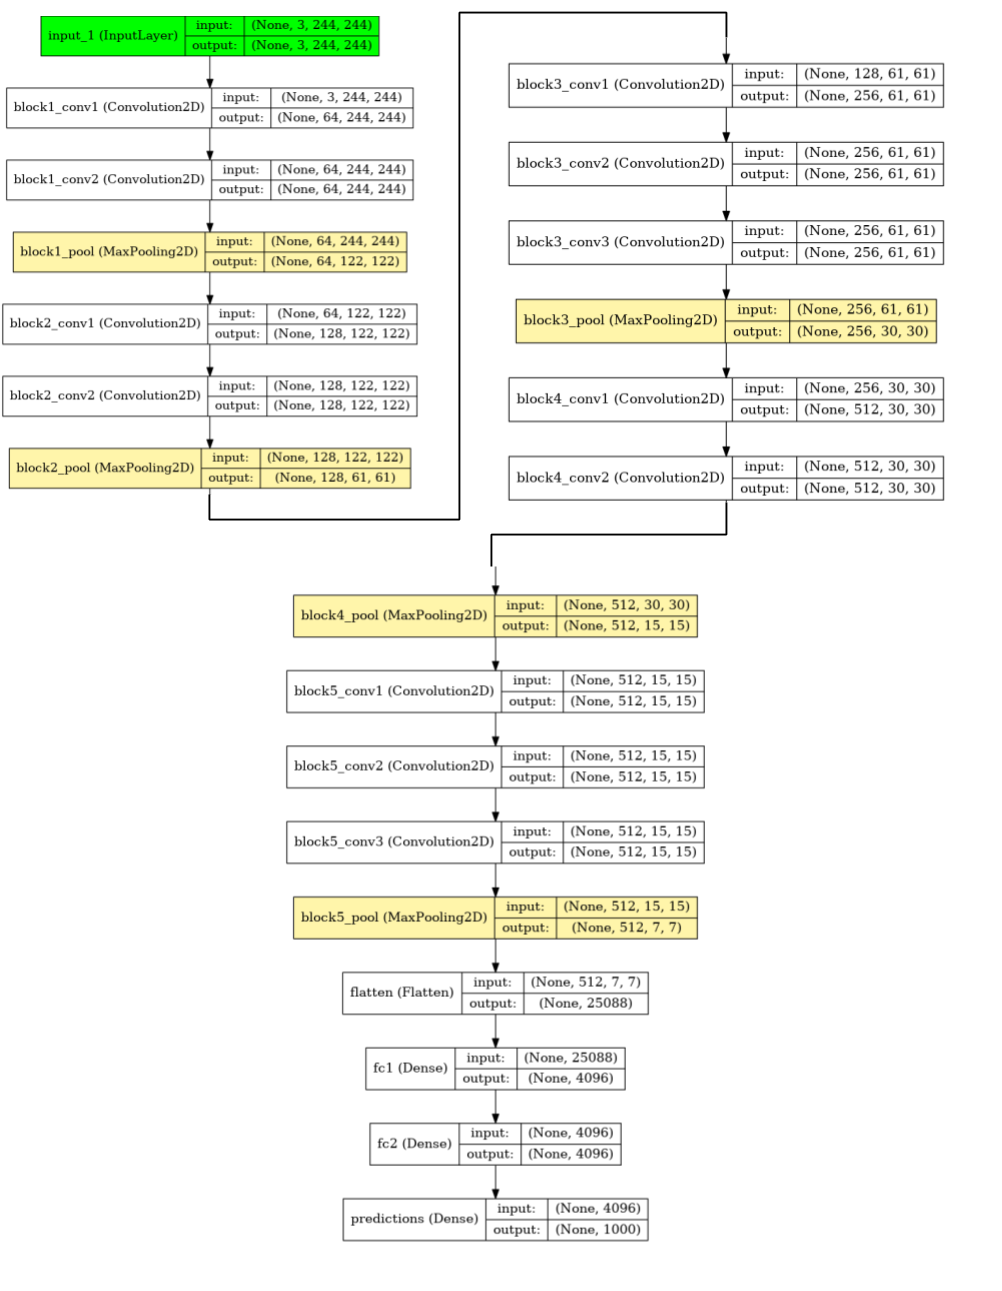
\includegraphics[width=0.9\textwidth]{./images/chapter5/vgg16.png}
  \caption[Πλήρες μορφή του δικτύου VGG16 της υλοποίησης]{Πλήρες μορφή του δικτύου VGG16 της υλοποίησης}
  \label{fig:vgg16}
\end{figure}

%% --------------------------------------------------------------------------
%\subsection{GoogleNet aka Inception-V1}

%\textbf{Να το προσθέσουμε και αυτό?}

%% --------------------------------------------------------------------------
\subsection{YOLO Net}

Το δίκτυο YOLO (You Only Look Once), είναι το πρώτο μοντέλο νευρωνικού δικτύου
συνέλιξης το οποίο προσπαθεί να επιλύσει το πρόβλημα της ταυτόχρονης αναγνώρισης
και εντοπισμού αντικειμένων σε εικόνες, με ένα προς-τα-εμπρός πέρασμα (forward pass).
Η ιδιαιτερότητά του είναι ότι αντιμετωπίζει το πρόβλημα σαν ένα πρόβλημα
regression και όχι classification.

Μία ακόμη ιδιαιτερότητα του συγκεκριμένου δικτύου είναι ότι θέτει σαν απαίτηση
την εφαρμογή του σε προβλήματα πραγματικού χρόνου και άρα στοχεύει κυρίως
στην ταχύτητα της αναγνώρισης. Φυσικά αυτό έχει σαν αποτέλεσμα την μείωση στην ακρίβεια
αναγνώρισης, η οποία είναι χαμηλότερη σε σχέση με άλλα μοντέλα, όπως για παράδειγμα τα δίκτυα
Fast-RCNN \cite{DBLP:journals/corr/Girshick15}, Overfeat και DetectorNet.

Η έξοδος του δικτύου αντιστοιχεί τόσο στις κλάσεις των αντικειμένων
που αναγνωρίστηκαν, καθώς και στις συντεταγμένες όπου και εντοπίστηκε.

\begin{figure}[!ht]
  \centering
  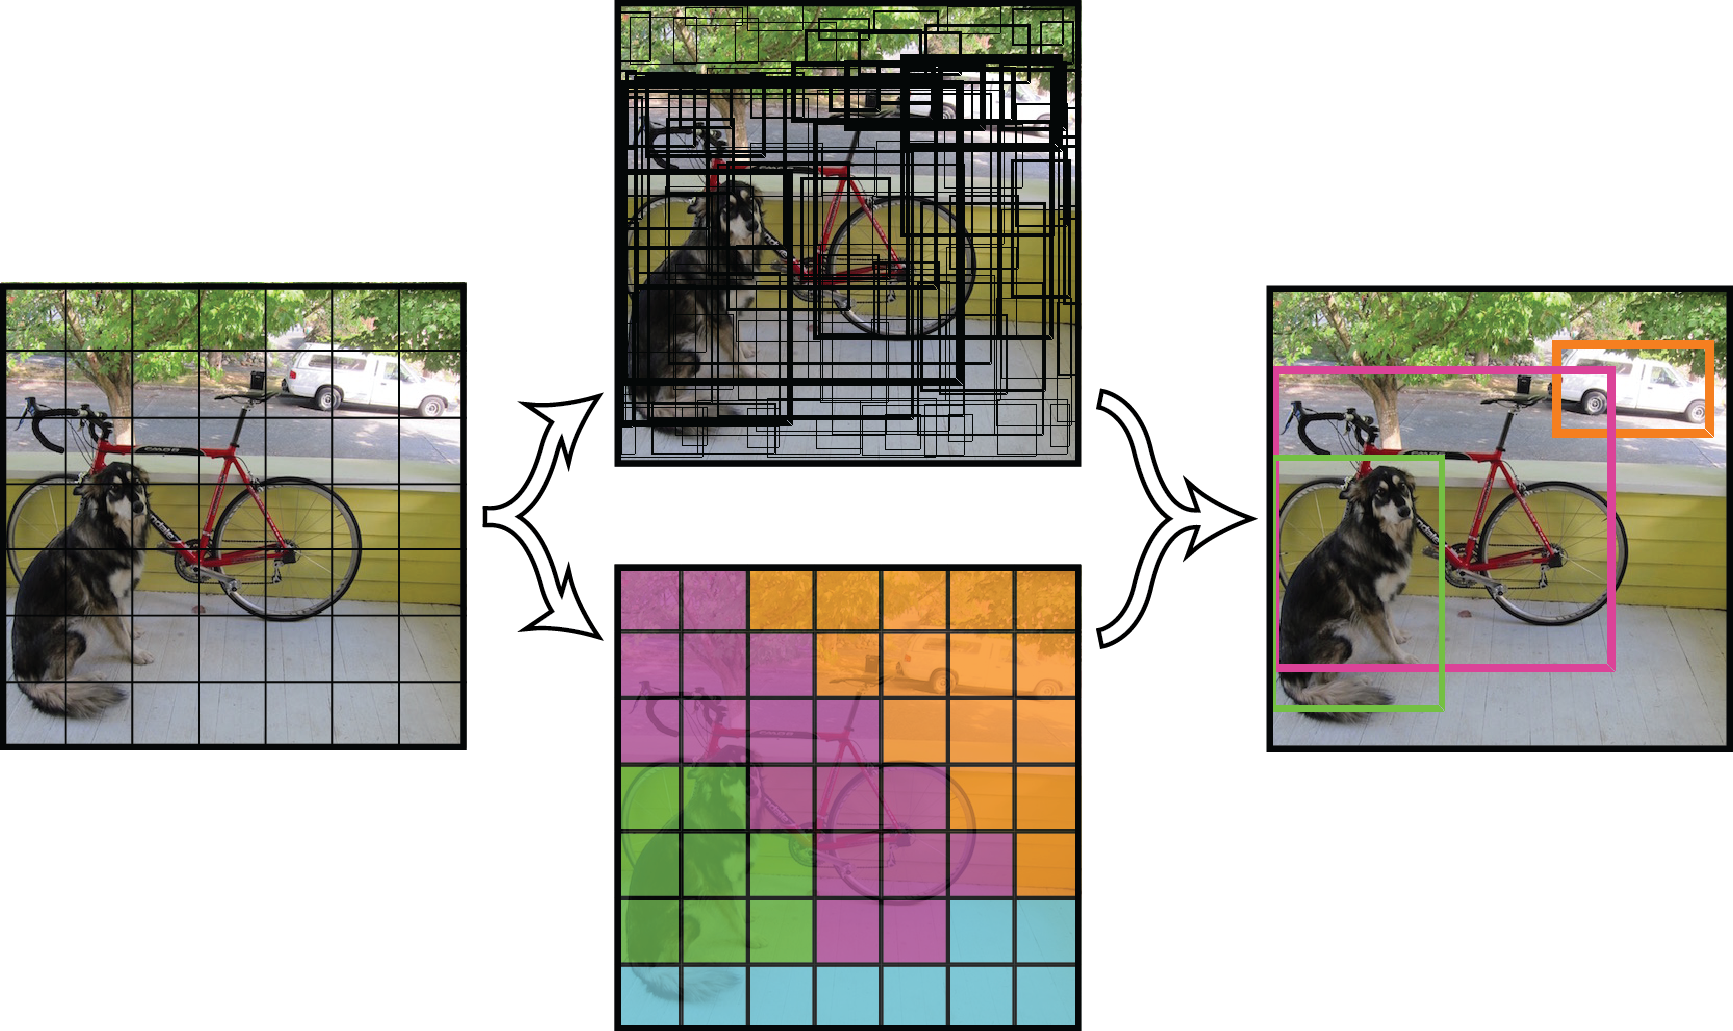
\includegraphics[width=0.8\textwidth]{./images/chapter5/yolonet_from_paper_1.png}
  \caption[Παράδειγμα τρόπου λειτουργίας του δικτύου YOLO]{Παράδειγμα τρόπου λειτουργίας του δικτύου YOLO}
  \label{fig:yolonet_from_paper}
\end{figure}

Το βασικό μοντέλο του δικτύου YOLO έχει την δυνατότητα να επεξεργάζεται εικόνες με ταχύτητα
\emph{45 fps} χρησιμοποιώντας μονάδα GPU (Nvidia Titan X).

Λόγω της ιδιαιτερότητας του συγκεκριμένου δικτύου, όσον αφορά τον τρόπο προσέγγισης του προβλήματος της ταυτόχρονης
αναγνώρισης και εντοπισμού των αντικειμένων, θεωρούμε σημαντικό να αναφέρουμε
και να εξηγήσουμε τον τρόπο λειτουργίας του.
Το πρώτο βήμα είναι να χωρίσει την εικόνα εισόδου σε ένα πλέγμα διαστάσεων $S \times S$
(αριστερή εικόνα στο \autoref{fig:yolonet_from_paper}).
Κάθε κελί του πλέγματος προβλέπει $B$ οριοθετημένα πλαίσια (bounding boxes) μαζί με ένα σκορ
"εμπιστοσύνης" για το κάθε πλαίσιο (πάνω μεσαία εικόνα στο \autoref{fig:yolonet_from_paper}).
Το σκορ εμπιστοσύνης ερμηνεύεται ως η βεβαιότητα
να ανήκει ένα αντικείμενο στο συγκεκριμένο πλαίσιο μαζί με την ακρίβεια ότι
το συγκεκριμένο αντικείμενο ανήκει σε αυτό το πλαίσιο. Η μαθηματική έκφραση
ορίζεται ως:
\begin{equation*}
  confidence = P(object | box = \imath) * IOU_{pred}^{truth}
\end{equation*}
Από την πιο πάνω μαθηματική έκφραση καταλαβαίνουμε ότι σε περίπτωση που
σε ένα κελί δεν υπάρχει αντικείμενο, το σκορ εμπιστοσύνης μηδενίζεται.
Επίσης, κάθε κελί του πλέγματος προβλέπει και τις πιθανότητες της κλάσης
του αντικειμένου, $P(class_{\imath} | object)$
(κάτω μεσαία εικόνα στο \autoref{fig:yolonet_from_paper}).

Χρησιμοποιώντας τις 2 αυτές μαθηματικές εκφράσεις των υπό-συνθήκη πιθανοτήτων,
καταλήγουμε στην σχέση
\begin{equation*}
  \begin{aligned}
    class-confidence = {} & P(class_{\imath} | object) * P(object | box = \imath) * IOU_{pred}^{truth} = \\
                          & P(class_{\imath}) * IOU_{pred}^{truth}
  \end{aligned}
\end{equation*}
η οποία μας δίνει το σκορ εμπιστοσύνης για μία συγκεκριμένη κλάση.

Κάθε οριοθετημένο πλαίσιο αποτελείται από πέντε προβλέψεις; $x, y, w, h$ και
το σκορ εμπιστοσύνης. Τα $x$ και $y$ αντιστοιχούν στις συντεταγμένες του
κέντρου του πλαισίου ενώ οι τιμές των $w$ και $h$ αναφέρονται στο
μήκος και το πλάτος του.

Τέλος, οι προβλέψεις στην έξοδο του δικτύου φαίνονται σαν ένας όγκος
διαστάσεων
\begin{equation*}
  S \times S \times (B * 5 + C)
\end{equation*}

Το πλήρες μοντέλο YOLO αποτελείτε από 24 επίπεδα συνέλιξης και 2 πλήρως
συνδεδεμένα.

Πέρα από το πλήρες μοντέλο, έχει σχεδιαστεί και εκπαιδευτεί, από την ίδια ομάδα ερευνητών, ένα μοντέλο
με παρόμοιο τρόπο λειτουργίας αλλά με πολύ λιγότερα επίπεδα συνέλιξης και άρα πιο
γρήγορο στην εκτέλεση (Tiny/Fast YOLO). Το TinyYOLO αποτελείτε από 9 επίπεδα
συνέλιξης και 2 πλήρες συνδεδεμένα. Σε όλα τα επίπεδα εκτός του τελευταίου
χρησιμοποιείται η συνάρτηση ενεργοποίησης LeakyReLU που παρουσιάστηκε στο \autoref{sec:theory_cnn}.

Η υλοποίηση μας στηρίχτηκε στην αντίστοιχη του μοντέλου Tiny-YOLO που έγινε από
την αντίστοιχη ερευνητική ομάδα \footnote{Βασική υλοποίηση του δικτύου YOLO: \url{http://pjreddie.com/darknet/}}
\cite{darknet13}.

Θεωρούμε σημαντικό να αναφέρουμε ότι αρχικά προσπαθήσαμε να τρέξουμε την βασική υλοποίηση,
η οποία είναι γραμμένη σε γλώσσα προγραμματισμού \emph{C}, ανεπιτυχώς.
Η εκτέλεση του προγράμματος υλοποίησης του μοντέλου Tiny-YOLO εμφανίζει σφάλματα
τύπου \emph{segmentation fault}.

\section{Βελτιστοποίηση των εργαλείων λογισμικού στο Jetson TK1}
\label{sec:implementations_jetson}

Στο \autoref{sec:jetson_tk1} είχαμε αναφέρει ότι η πλατφόρμα διαθέτει
λειτουργικό \emph{Linux4Tegra} το οποίο είναι ουσιαστικά διανομή Ubuntu 14.04
με εγκατεστημένους τους απαραίτητους drivers για το συγκεκριμένο σύστημα.

%προτού ξεκινήσουμε τις υλοποίησεις χρειάστηκε να εγκαταστήσουμε
%τα περισσότερα εργαλεία κατευθείαν πάνω στο μηχάνημα (build from source), για να αποφύγουμε
%την εγκατάστασή pre-compiled λογισμικού. Ο λόγος, όπως και θα φανεί στο \autoref{chapter:experiments},
%είναι ότι η απόδοση των συγκεκριμένων εργαλείων εξαρτάται τόσο από τις
%βιβλιοθήκες που θα χρησιμοποιηθούν για πράξεις γραμμικής άλγεβρας,
%όσο και από τις βελτιστοποιήσεις που γίνονται από τον μεταγλωττιστή κατά την
%διάρκεια της μεταγλώττισης του εκάστοτε πηγαίου κώδικά.

Ένα από τα πρώτα βήματα ήταν να απ-εγκαταστήσουμε από το λειτουργικό το
γραφικό περιβάλλον, για να περιορίσουμε την κατανάλωση μνήμης αφού η μνήμη
του ενσωματωμένου συστήματος Jetson TK1 είναι περιορισμένη στα 2 Gigabytes
και μάλιστα είναι κοινή μεταξύ των μονάδων GPU και CPU (shared memory).
Το γραφικό περιβάλλον Gnome
το οποίο είναι προεγκατεστημένο στην διανομή Linux4Tegra μετρήθηκε στα 114 Megabytes.
Το Jetson TK1 συνδέθηκε
μέσω θύρας ethernet στο δίκτυο ενός σταθερού υπολογιστή και έτσι ο χειρισμός
του έγινε μέσω καναλιού ssh\footnote{SSH: Secure Shell \href{https://tools.ietf.org/html/rfc4254}{{https://tools.ietf.org/html/rfc4254}}},
κερδίζοντας έτσι 114 Megabytes σε μνήμη. Αυτό το κέρδος, όπως θα φανεί
αργότερα, έπαιξε σημαντικό ρόλο, καθώς τα νευρωνικά δίκτυο που υλοποιήθηκαν
απαιτούν αρκετή μνήμη κατά την διάρκεια εκτέλεσής τους (της τάξης των Gigabytes).

Στην συνέχεια εγκαταστήσαμε τις βιβλιοθήκες CUDA και cuDNN για να εκμεταλλευτούμε
την υπολογιστική ισχύ της μονάδας GPU. Ο οδηγός για την εγκατάσταση βρίσκεται
στο %\href{http://elinux.org/Jetson_TK1}{http://elinux.org/Jetson_TK1}.
Επιπλέον έχουν γραφεί scripts σε \emph{Bash} για αυτόματη εγκατάσταση, τα
οποία είναι διαθέσιμα στο \emph{Github} στον σύνδεσμο %?????
%\href{https://github.com/klpanagi/Thesis/tree/master/jetson-tk1/}{https://github.com/klpanagi/Thesis/tree/master/jetson-tk1/}.

Ένα μεγάλο μέρος της συνεισφοράς της παρούσας διπλωματική εργασίας
ήταν να γίνουν βελτιστοποιήσεις σε επίπεδο λογισμικού των εργαλείων που χρησιμοποιήθηκαν
για το συγκεκριμένο μηχάνημα.

Αρχικά, ακολουθήσαμε τις οδηγίες για εγκατάσταση των εργαλείων \emph{numpy, scipy, Theano και Keras}
χρησιμοποιώντας τον επίσημο διαχειριστή πακέτων για Python, \emph{pip}.
Τα πρώτα αποτελέσματα σε χρόνους εκτέλεσης πράξεων γραμμικής άλγεβρας ήταν
απαγορευτικά (σχεδόν μία τάξη μεγέθους κάτω από το αναμενόμενο).
Τόσο η βιβλιοθήκη Theano, όσο και η numpy, χρησιμοποιούν εξωτερικές βιβλιοθήκες
για πράξεις γραμμικής άλγεβρας, οι οποίες ονομάζονται BLAS (Basic Linear Algebra Subprograms).

Καταλάβαμε ότι το πρόβλημα ήταν στους υπολογισμούς πράξεων γραμμικής άλγεβρας,
αφού σχεδόν όλες οι μαθηματικές εκφράσεις που εκτελούνται σε ένα
νευρωνικό δίκτυο είναι πράξεις πινάκων και εκτελέστηκε profiling των
ρουτινών BLAS χρησιμοποιώντας και τις τρεις βιβλιοθήκες που είναι διαθέσιμες για
επεξεργαστές ARM οι οποίες είναι οι εξής:
\begin{itemize}
  \item{libblas-dev + liblapack3 + libumfpack5.6.2: Προ-εγκατεστημένες στην διανομή Linux4Tegra}
  \item{ATLAS: Ανοικτού κώδικα}
  \item{OpenBLAS: Ανοικτού κώδικα}
\end{itemize}

Τόσο η βιβλιοθήκη ATLAS, όσο και η OpenBLAS, μεταγλωττίστηκαν από τον πηγαίο κώδικά τους,
λαμβάνοντας έτσι υπόψη τις απαραίτητες βελτιστοποιήσεις κατά την διαδικασία
της μεταγλώττισης. 
Συγκεκριμένα ορίσαμε στον μεταγλωττιστή να χρησιμοποιήσει την αρχιτεκτονική του
συγκεκριμένου επεξεργαστή (armv7) και τις μονάδες
NEON που διαθέτει, για τον υπολογισμό πράξεων με αριθμούς κινητής %?? what are NEON? ref or comment
υποδιαστολής \emph{ARM Cortex A15}. Επίσης ορίσαμε η εκτέλεση των ρουτινών
BLAS να γίνεται με πολυνηματικό τρόπο (4 threads).

Στην συνέχεια μετρήθηκε η απόδοση σε χρόνο εκτέλεσης των εξής ρουτινών BLAS:
\begin{itemize}
  \item{Εσωτερικό γινόμενο δύο διανυσμάτων με 1000 στοιχεία το καθένα}
  \item{Εσωτερικό γινόμενο δύο πινάκων διαστάσεων $1000 \times 1000$}
  \item{Αντιστροφή πίνακα διαστάσεων $1000 \times 1000$}
  \item{Υπολογισμός διακρίνουσας πίνακα διαστάσεων $1000 \times 1000$}
  \item{Υπολογισμός ιδιοτιμών πίνακα διαστάσεων $2000 \times 1000$}
  \item{Υπολογισμός ιδιοδιανυσμάτων πίνακα διαστάσεων $1500 \times 1500$}
\end{itemize}
Εκτελέστηκε κάθε μία από τις πιο πάνω ρουτίνες για 1000 επαναλήψεις και λήφθηκε
η μέση τιμή του χρόνου εκτέλεσης.
Οι καλύτεροι χρόνοι λήφθηκαν χρησιμοποιώντας την βιβλιοθήκη OpenBLAS.
Τα συγκριτικά αποτελέσματα μεταξύ της βιβλιοθήκης OpenBLAS και της προεγκατεστημένης
έχουν ως εξής: % add times instead of X times. Also put them in a table
\begin{itemize}
  \item{Εσωτερικό γινόμενο πινάκων: $\times 18$}
  \item{Εσωτερικό γινόμενο διανυσμάτων: καμία διαφορά}
  \item{Αντιστροφή πίνακα: $\times 11.5$}
  \item{Υπολογισμός διακρίνουσας πίνακα: $\times 9.6$}
  \item{Υπολογισμός ιδιοτιμών πίνακα: $\times 8.5$}
  \item{Υπολογισμός ιδιοδιανυσμάτων πίνακα: $\times 3.4$}
\end{itemize}
Αντίστοιχα, χρησιμοποιώντας την βιβλιοθήκη ATLAS πήραμε τα εξής αποτελέσματα:
\begin{itemize}
  \item{Εσωτερικό γινόμενο πινάκων: $\times 16$}
  \item{Εσωτερικό γινόμενο διανυσμάτων: $\times 1.5$}
  \item{Αντιστροφή πίνακα: $\times 10.2$}
  \item{Υπολογισμός διακρίνουσας πίνακα: $\times 7.4$}
  \item{Υπολογισμός ιδιοτιμών πίνακα: $\times 7.8$}
  \item{Υπολογισμός ιδιοδιανυσμάτων πίνακα: $\times 3.4$}
\end{itemize}

Αφού καταλήξαμε στην χρησιμοποίηση της βιβλιοθήκης OpenBLAS, συνεχίσαμε
με την μεταγλώττιση από πηγαίο κώδικα των βιβλιοθηκών numpy, scipy και Theano,
οι οποίες εκτελούν τις πράξεις BLAS, ορίζοντας αυτή την φορά στον μεταγλωττιστή
να χρησιμοποιήσει την συγκεκριμένη βιβλιοθήκη αντί της προ-εγκατεστημένης (link against shared library).

Τέλος, εγκαταστήσαμε στον Jetson TK1 την βιβλιοθήκη \emph{CNMeM}
\footnote{\href{https://github.com/NVIDIA/cnmem}{https://github.com/NVIDIA/cnmem}},
η οποία έχει αναπτυχθεί από την Nvidia και χρησιμοποιείται για την εκ των προτέρων
δέσμευση μνήμης σε μονάδες GPU που υποστηρίζουν CUDA.
Όπως θα φανεί στο επόμενο κεφάλαιο, η εκ των προτέρων δέσμευση μνήμης
επιταχύνει τον χρόνο εκτέλεσης. Ωστόσο απαιτεί σωστή ρύθμιση για να
αποφευχθούν περιπτώσεις δέσμευσης περισσότερης μνήμης από όση το
πρόγραμμα εκτέλεσης χρειάζεται.

Τέλος, είναι σημαντικό να αναφέρουμε ότι όλες οι προαναφερθέντες διαδικασίες εγκατάστασης των
εργαλείων λογισμικού καθώς και τα πειράματα που εκτελέσθηκαν περιγράφονται πλήρως στον
ιστοχώρο: %
\\

\href{https://github.com/klpanagi/Thesis/tree/master/jetson-tk1}{https://github.com/klpanagi/Thesis/tree/master/jetson-tk1}





